\chapter{Schiere di antenne}

	Vedremo in questo capitolo come combinare in modo opportuno una serie di antenne per migliorare le prestazioni del nostro ricevitore.

\section{Schiera di antenne isotrope}
	Il primo caso che analizzeremo è quello di una serie lineare ed equispaziata di antenne isotrope, ovvero antenne che irradiano in modo uniforme in tutte le direzioni.

	Questa semplificazione permette di considerare le proprietà del posizionamento delle antenne nell'\emph{array} astraendo dalle caratteristiche specifiche delle varie antenne.

	\begin{figure}[ht]
		\centering
		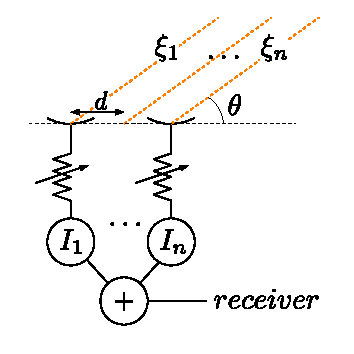
\includegraphics{img/schiera_antenne.pdf}
		\caption{Le antenne della schiera sono alimentate dalle correnti $I_i$ e ricevono il segnale dal campo lontano con sfasamenti diversi $\xi_i$.}
		\label{fig:schiera}
	\end{figure}

	Dallo schema elettrico in figura \ref{fig:schiera} si può facilmente calcolare il segnale in arrivo al ricevitore, definito come \gls{af}.

	\begin{esp} \label{eq:array_factor}
		AF = \sum_{i=1}^n I_i e^{\jmath \xi_i}
			\stackrel{(*)}{=} \sum_{i=1}^n I_i ~ e^{\jmath (i-1) \beta d \cos \theta}
	\end{esp}
	dove in (*) si calcola la differenza di cammino tra i vari percorsi.

	\subsection{Schiere fasate}
		Un caso particolare, ma di notevole interesse, sono le \emph{schiere fasate}, array in cui le correnti hanno modulo uguale e sfasamento $\alpha$. 
		Il calcolo dell'\gls{af} per questa scelta dei parametri si semplifica ulteriormente.
			
		\begin{esp}
				AF 
				& = \sum_{k=0}^{n-1} I_k ~ e^{\jmath k \beta d \cos \theta} \\
				& \stackrel{(1)}{=}  \sum_{k=0}^{n-1} A_k ~ e^{\jmath k (\beta d \cos \theta + \alpha)}
					\stackrel{(2)}{=} \sum_{k=0}^{n-1} ~ A_k e^{\jmath k \psi} \\
				& = A_o \sum_{k=0}^{n-1} e^{\jmath k \psi}
					\stackrel{(3)}{=} A_o 
						\left( \frac{ 1 - e^{\jmath n \psi} }{ 1 - e^{\jmath \psi} } \right) \\
				& = A_o 
						~ \frac{ e^{\jmath \frac{n}{2} \psi} }{ e^{\jmath \psi} } 
						\left( \frac{ e^{\jmath \frac{n}{2} \psi} - e^{- \jmath \frac{n}{2} \psi} }{ e^{\jmath \psi} - e^{-\jmath \psi} } \right) \\
				& = A_o
					\left( \frac{ \sin(\frac{n}{2} \psi) }{ \sin(\frac{\psi}{2}) } \right) 
					~ e^{\jmath \frac{n-1}{2} \psi}
			\end{esp}
		dove 
		\begin{itemize}
			\item[(1)] $I_k$ viene scomposto in modulo e fase come $A_k ~ e^{\jmath k \alpha}$
			\item[(2)] l'angolo $\psi$ è definito, per semplificare la notazione, come la somma di tutti gli sfasamenti per l'antenna $k$-esima
			\item[(3)] viene utilizzata la formula per il calcolo della serie geometrica troncata.
		\end{itemize}
		
		\subsubsection{Regione di visibilità}
			I valori validi di $\theta$, ovvero l'inclinazione dell'onda incidente rispetto all'array, sono nell'intervallo $[0, \pi]$: le proprietà dell'array per i valori opposti sono ottenute semplicemente per simmetria.
			
			Questo induce dei limiti nell'angolo $\psi$: il range di valori validi per questo angolo è detto \emph{regione di visibilità}.
			\begin{equation} \begin{gathered}
			0 \le \theta \le \pi \\
			-\beta d \le \beta d \cos \theta \le \beta d \\ 
			\alpha - \beta d \le \psi \le \alpha + \beta d 
			\end{gathered} \end{equation}
		
		\subsubsection{Massimo di radiazione}
			Il massimo delle capacità dell'antenna si ha per $\psi = 0$, che corrisponde all'angolo (o agli angoli) $\theta_o$ nella regione di visibilità per cui $\beta d \cos \theta_o = -\alpha$.
			
			\begin{esp}
				|AF(\psi = 0)| 
					& = A_o 
						~ \left( \lim_{\psi \to 0} \frac{ \sin(\frac{n}{2} \psi) }{ \sin(\frac{\psi}{2}) } \right)
						~ \left| \frac{ e^{\jmath \frac{n-1}{2} \psi} }{ e^{\jmath \psi} } \right| 
						= A_o \cdot n \cdot 1 = A_o \cdot n
			\end{esp}

			Questa osservazione ci permette di calcolare il pattern di radiazione dell'array, definito come il modulo dell'\gls{af} normalizzato al suo valor massimo.
			
			\begin{equation} \label{eq:array_pattern}
				F(\theta) 
					= \frac{1}{n} ~ \frac{\sin(\frac{n}{2} \psi) }{ \sin( \frac{\psi}{2} ) }
					= \frac{1}{n} ~ \frac{
						\sin \left(
							\frac{n}{2} (\beta d \cos \theta + \alpha)
						\right) 
					}{
						\sin \left(
							\frac{(\beta d \cos \theta + \alpha)}{2}
						\right)
					}
			\end{equation}
			
		\subsubsection{Minimo di radiazione}
			Osservando l'equazione \ref{eq:array_pattern} si può notare che gli zeri del campo lontano si hanno per valori di $\psi$ che annullano il numeratore, ma non il denominatore.
			
			\begin{esp}
				\frac{1}{n} ~ \frac{\sin(\frac{n}{2} \psi) }{ \sin( \frac{\psi}{2} ) } = 0
				\Leftrightarrow 
					\frac{n}{2} \psi = \pm m \pi \quad \forall m \neq 0
			\end{esp}
			
		\subsubsection{Lobi secondari}
			Lobi secondari troppo pronunciati possono minare la direttività dell'array: per questo motivo è utile calcolarne l'entità.
			
			Cerco quindi i massimi della funzione \gls{af}.
			
			\begin{esp}
				\deriv{AF}{\psi} 
				& = \deriv{}{\psi} \left(
						\frac
							{ \sin(\frac{n}{2} \psi) }
							{ \sin( \frac{\psi}{2} ) }
					\right) \\
				& = \frac{1}{\sin^2 \frac{\psi}{2}} \left[
					\cos \left(\frac{n}{2} \psi \right) \frac{n}{2} \sin\left( \frac{\psi}{2} \right) 
					- \sin \left(\frac{n}{2} \psi \right) \cos\left( \frac{\psi}{2} \right)
					\right]
				 = 0
			\end{esp} 
			
			Per valori di $n$ grandi (indicativamente maggiori di 10), si può compiere questa semplificazione.
			
			\begin{esp}
				\cos \left(\frac{n}{2} \psi \right) \sin\left( \frac{\psi}{2} \right)
				= \frac{2}{n} \sin \left(\frac{n}{2} \psi \right) \cos\left( \frac{\psi}{2} \right)
				\simeq 0 \quad \forall n \to +\infty
				 = 0
			\end{esp} 
			
			Le soluzioni dell'equazione precedente sono quindi
			\begin{equation*}
				\begin{dcases}
					\psi = 0, \pi 
						& \text{non accettabili, perché punti di massimo} \\
					\psi = \pm \frac{\pi}{n} (2p + 1) \quad \forall p \in \mathbb{N}
						& \text{validi se rientrano nel range di visibilità}
				\end{dcases}
			\end{equation*}

			Ottenute le posizioni di massimi e minimi in $\psi$ è possibile calcolare attraverso la funzione $AF(\psi)$ il \emph{Side Lobe Level}, che misura il rapporto tra lobi primari e secondari.

	\subsection{Tipologie di schiere lineari fasate}
		Come si può notare dalla definizione di $\psi$, il massimo che si ha per $\psi = 0$ corrisponde ad un valore di $\theta$ che è funzione dello sfasamento delle correnti $\alpha$.
		
		La possibilità di spostare il lobo principale in modo elettronico, senza quindi variazioni meccaniche della schiera, è un punto di forza di questa tipologia di antenne perché le rende riconfigurabili ``al volo''.
		
		A seconda dei valori di $\alpha$, le schiere lineari fasate si dividono in 
		\begin{esp*}
			\alpha = 0 
				& \implies \theta_o = \frac{\pi}{2} 
				& \text{schiere \emph{broadside}} \\
			\alpha = \pm \beta d 
				& \implies \theta_o = 0 \land \theta_o = \pi 
				& \text{schiere \emph{endfire}} \\
		\end{esp*}

\section{Schiera di antenne non isotrope}
	

		